\def\CTeXPreproc{Created by ctex v0.2.5, don't edit!}\documentclass[12pt]{article}
\usepackage{mathrsfs}
\usepackage{amsfonts}
\textwidth 160mm \textheight 240mm \hoffset -1.4 cm \voffset -1.6cm
\usepackage[centertags]{amsmath}
\usepackage{indentfirst}
\usepackage{latexsym}
\usepackage{amssymb}
\usepackage{epsfig}
\usepackage{pst-all}
\usepackage{epsfig}
\usepackage{graphicx,color}
\usepackage{picinpar}
\usepackage{subfigure}
\usepackage{bm}
\usepackage{makeidx,ifthen}
\usepackage{amsmath}

\newcommand{\updown}[2]{\underset{#2}{#1}\,}
%\newcommand{\bm}[1]{\mbox{\boldmath{$#1$}}}

\newtheorem{defn}{Definition}[section]
%\newtheorem{thm}{Theorem}[section]
\newtheorem{thm}{Theorem}
%\newtheorem{cor}[thm]{Corollary}
\newtheorem{cor}{Corollary}
%\newtheorem{lem}[thm]{Lemma}
\newtheorem{lem}{Lemma}
\newtheorem{prop}[thm]{Proposition}
\newtheorem{rem}{Remark}[section]
\numberwithin{equation}{section}
\renewcommand{\baselinestretch}{1.4}

%------------------------------------
\newcommand{\thmref}[1]{Theorem~\ref{#1}}
\newcommand{\propref}[1]{Proposition~\ref{#1}}
\newcommand{\lemref}[1]{Lemma~\ref{#1}}
\newcommand{\corref}[1]{Corollary~\ref{#1}}
\newcommand{\remref}[1]{Remark~\ref{#1}}
\newcommand{\examref}[1]{Example~\ref{#1}}
\newcommand{\secref}[1]{Section~\ref{#1}}
\newcommand{\ssecref}[1]{\S\ref{#1}}
\newcommand{\chapref}[1]{Chapter~\ref{#1}}
\newcommand{\eqnref}[1]{(\ref{#1})}
\newcommand{\figref}[1]{Figure~\ref{#1}}
\newcommand{\appref}[1]{Appendix~\ref{#1}}
\newcommand{\assref}[1]{Assumption~\ref{#1}}
\newcommand{\defref}[1]{Definition~\ref{#1}}
%-------------------------------------------

\graphicspath{{Figures-Inv/}}

\begin{document}


\title{Optimal monetary policy with interest variances in the objective function}



\maketitle
%------------------------------------------------------------------------------------------
%%------------------------------------------------------------





\section{Optimal Monetary Policy}
\label{sec:MonPol}
%BLE are characterized by persistence amplification, with much higher persistence in output and inflation than in the exogenous driving forces, and volatility amplification, with the variances at the BLE much higher than at the REE in most cases.  This leaves an important question for the optimal values of Taylor rule parameters at the BLE. As shown in Boehm and House (2014), at the REE when the output gap and
%inflation are observed without error, it is typically optimal to respond infinitely strongly to observed deviation from the central bank's targets, while with measurement error the optimal Taylor rule coefficients are finite.
%How do the optimal values of Taylor rule parameters differ between the BLE and REE? In this section we try to answer this question.

Similar to Boehm and House (2014), Evans and Honkapohja (2003) and Woodford (2003), we assume that the central bank wishes to minimize an expected discounted sum of weighted squared inflation and output gap
\begin{equation}
(1-\vartheta)E\Big[\Sigma_{t=0}^\infty \vartheta^t[\pi_t^2+\omega_yy_t^2+\omega_r r_t^2] \Big]=\omega\sigma_\pi^2+\omega_y\sigma_y^2+\omega_r\sigma_r^2,\label{varobj}
\end{equation}
where $\omega$ is the relative weight that the central bank places on inflation. %From the equations (\ref{varyapp}) and (\ref{varpiapp}) in Appendix \ref{acfnkc},
Based on our calculation
\begin{eqnarray}
\sigma_y^2&=&\frac{\widetilde{g}_1}{(1+\gamma\varphi\phi_\pi+\varphi\phi_y)^2(1-\rho^2)(1-\rho\lambda_1)(1-\rho\lambda_2)(1-\lambda_1^2)(1-\lambda_2^2)(1-\lambda_1\lambda_2)}, \label{varyc}\\
\sigma_\pi^2&=&\frac{\widetilde{g}_2}{(1+\gamma\varphi\phi_\pi+\varphi\phi_y)^2(1-\rho^2)(1-\rho\lambda_1)(1-\rho\lambda_2)(1-\lambda_1^2)(1-\lambda_2^2)(1-\lambda_1\lambda_2)}, \label{varpic}\\
\sigma_r^2&=&\phi_y^2\sigma_y^2+\phi_\pi^2\sigma_\pi^2+2\phi_y\phi_\pi E(y\pi),\label{varrc}
\end{eqnarray}
where $\widetilde{g}_1$, $\widetilde{g}_2$, $\lambda_1$, $\lambda_2$ are given by the equations (\ref{gyvar}), (\ref{gpivar}), (\ref{lambdatr}) and (\ref{lambdade}), and
\begin{eqnarray*}
E(y\pi)&=&\Big(-\sigma_1^2\gamma\big(-(1+\gamma\varphi\phi_\pi+\varphi\phi_y)(1+\gamma\varphi\phi_\pi+\varphi\phi_y+\beta_1^2\rho)+\beta_2^4\lambda(1+\gamma\varphi\phi_\pi\\
&&+\varphi\phi_y+\beta_1^2\rho)(\lambda+\gamma\varphi+\lambda\varphi\phi_y)+\beta_2^2\rho[\beta_1^4\lambda+\beta_1^2\lambda\rho(1+\gamma\varphi\phi_\pi+\varphi\phi_y)+\gamma\varphi\\
&&(-1+\lambda \phi_\pi)(1+\gamma\varphi\phi_\pi+\varphi\phi_y)]-\beta_1^2\beta_2^6\lambda^2\rho(\beta_1^2\lambda+\rho(\lambda+\gamma\varphi+\lambda\varphi\phi_y))\big)+\sigma_2^2\varphi\\
&&\big(-\phi_\pi(1+\gamma\varphi\phi_\pi+\varphi\phi_y)[-\beta_1^4-\beta_1^2\gamma\rho\varphi\phi_\pi+(1+\varphi\phi_y)(1+\gamma\varphi\phi_\pi+\varphi\phi_y)]+\beta_1^2\beta_2^6\lambda\rho\\
&&[-\gamma\varphi(-\beta_1^2+\rho+\rho\varphi\phi_y)+\lambda\rho(\beta_1^4-(1+\varphi\phi_y)^2)]+\beta_2^4\big(\gamma\varphi(1-\beta_1^2\rho+\varphi\phi_y)(1+\gamma\varphi\phi_\pi\\
&&+\varphi\phi_y)+\lambda(-1+\beta_1^2\rho-\varphi(\gamma\phi_\pi+\phi_y))(\beta_1^4-(1+\varphi\phi_y)^2)+\beta_1^2\lambda^2\rho\phi_\pi(-\beta_1^4+\\
&&(1+\varphi\phi_y)^2)\big)+\beta_2^2\rho[-\beta_1^6\lambda\rho\phi_\pi+\beta_1^2\lambda\rho\phi_\pi(1+\varphi\phi_y)(1+\gamma\varphi\phi_\pi+\varphi\phi_y)-(-1+\lambda\phi_\pi)\\
&&(1+\varphi\phi_y)^2(1+\gamma\varphi\phi_\pi+\varphi\phi_y)+\beta_1^4(-1-\varphi(\gamma\phi_\pi+\varphi_y)+\lambda(\phi_\pi+\varphi\phi_\pi\phi_y))]\big)\Big)\Big/  \\
&& \Big((-1+\rho^2)(-1+\beta_1^2\beta_2^2\lambda-\varphi(\gamma\phi_\pi+\phi_y))(1+\beta_1^2\rho(-1+\beta_2^2\lambda\rho)+\gamma\varphi\phi_\pi+\varphi\phi_y\\
&&-\beta_2^2\rho(\lambda+\gamma\varphi+\lambda\varphi\phi_y))\big(\beta_1^4(-1+\beta_2^4\lambda^2)+2\beta_1^2\beta_2^2\gamma\varphi(-1+\lambda\phi_\pi)+(1+\gamma\varphi\phi_\pi+\varphi\phi_y)^2\\
&&-\beta_2^4(\lambda+\gamma\varphi+\lambda\varphi\phi_y)^2\big)\Big).
\end{eqnarray*}
In the following we study the optimal values  $(\phi_y^*, \phi_\pi^*)$ that minimize the central bank's loss function (\ref{varobj}) at the BLE, where $\beta_1^*$ and $\beta_2^*$ are at the behavioral learning equilibria.


\begin{figure}
    \begin{center}
     \includegraphics[width=3.2in]{optpolicy09.eps}
     \end{center}
   \caption{\label{opt09} Optimal policies at the BLE and at the REE. Parameters are: $\lambda=0.99, \varphi=1, \rho=0.5,\gamma=0.04,\sigma_1=1,\sigma_2=0.5$ and $\omega_y=0.1,\omega_r=0.05$.}
    \end{figure}


\begin{figure}
    \begin{center}
        \mbox{\subfigure[At the BLE ]
        {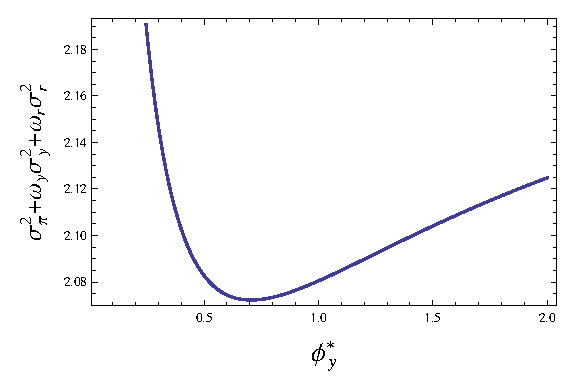
\includegraphics[width=3.2in]{varble09.eps}}\quad
        \subfigure[At the REE]
         {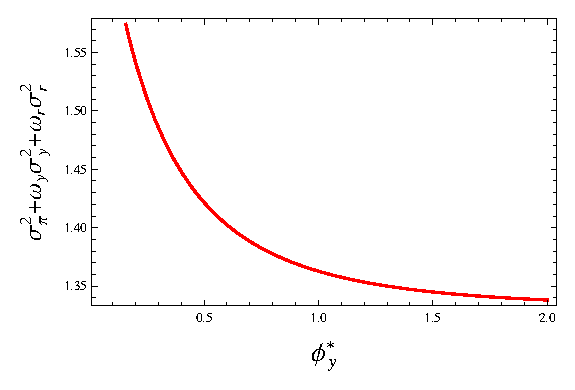
\includegraphics[width=3.2in]{varree09.eps}}}
   \end{center}
   \caption{\label{varopt09} Loss function along the optimal paths $(\phi_y^*, \phi_\pi^*)$ in Figure \ref{opt09} at the BLE (a) and REE (b). Parameters are:  $\lambda=0.99, \varphi=1, \rho=0.5,\gamma=0.04,\sigma_1=1,\sigma_2=0.5$ and $\omega_y=0.1,\omega_r=0.05$.}
    \end{figure}


As before in the benchmark we consider the parameters $\lambda=0.99, \varphi=1, \gamma=0.04, \rho=0.5, \sigma_1=1, \sigma_2=0.5$. We first consider the case $\omega_y=0.1,\omega_r=0.05$, that is, the central bank places relatively large weight on inflation. Interestingly, we find that the optimal Taylor rule coefficients $(\phi_y^*, \phi_\pi^*)$ are finite in this case\footnote{
We first select a policy parameter domain (e.g. $[0,100]\times[1,100]$) and define a lattice with some small step ($e.g. \,\,0.01$). Then for each lattice point $(\phi_y, \phi_\pi)$, we find the BLE $(\beta_1^*(\phi_y, \phi_\pi), \beta_2^*(\phi_y, \phi_\pi))$ and the corresponding central bank's loss function $\omega\sigma_\pi^2+\omega_y\sigma_y^2+\omega_r\sigma_r^2$ at the BLE. Finally we interpolate the loss function with respect to $(\phi_y, \phi_\pi)$ to find the finite optimal values. It is easy to get analytic expressions of REE and the corresponding variances. In contrast, it is impossible to obtain analytic expressions of the optimal policy parameters under BLE and  therefore we have to rely on numerical approximations. }.
As shown in Figure \ref{opt09}a, the corresponding optimal policy $(\phi_y^*, \phi_\pi^*)=(0.7058, 4.2228)$. %\footnote{In the case $\omega=0.7$, e.g., and the other parameters the same, the optimal policy $(\phi_y^*, \phi_\pi^*)=(6.699, 10.812)$.}.
This is different from REE, where there is no finite optimal policy here. In fact, from Figure \ref{opt09} it can be seen that in the case $\phi_y^*$ is small enough (i.e. $<0.7058$) the coefficients $\phi_y^*$ and $\phi_\pi^*$ lie on a manifold and the loss function (\ref{varobj}) decreases gradually along the manifold within the region, which is similar to REE but with higher $\phi_\pi^*$. However, differently in the case $\phi_y^*>0.7058$, the loss function (\ref{varobj}) starts to increase, while in the REE the loss function (\ref{varobj}) still decreases as shown in Figure~\ref{varopt09}. That is to say, there exist finite optimal Taylor rule coefficients at the BLE, but not at the REE. This is mainly because at the BLE the actual law of motion has higher volatility (especially for inflation) than at the REE in most cases and minimizing the loss function, i.e. minimizing the weighted variances of output gap and inflation, requires balancing the different responses in terms of policy parameters $(\phi_y, \phi_\pi)$.





\begin{figure}
    \begin{center}
        \mbox{\subfigure[Optimal policy ]
        {\includegraphics[width=3.2in]{optpolicyrho09.eps}}\quad
        \subfigure[Optimal manifold]
         {\includegraphics[width=3.2in]{optmanifrho.eps}}}
   \end{center}
   \caption{\label{optrho}  Optimal policies at the BLE with respect to $\rho$ (a) and corresponding optimal manifolds for three different $\rho$ (connection points of solid and dotted curves corresponding to finite optimal policies) (b). Parameters are: $\lambda=0.99, \varphi=1, \gamma=0.04,\sigma_1=1,\sigma_2=0.5$ and $\omega_y=0.1,\omega_r=0.05$.}
    \end{figure}

%In order to understand this in more detail, Figure \ref{varypi} shows plots of the (weighted) variances of output gap and inflation at the BLE as a function of $\phi_y$ and $\phi_\pi$. Figure \ref{varypi}a shows that the variance of output gap at the BLE decreases with respect to $\phi_y$ for given $\phi_\pi$, but increases as $\phi_\pi$ grows for given $\phi_y$. Similarly, Figure \ref{varypi}b suggests that the variance of inflation at the BLE decreases with respect to $\phi_\pi$, but increases as $\phi_y$ grows. That is, if the central bank tries to increase $\phi_y$ to reduce the variation in output gap, then it must endure higher variation in inflation or if the central bank tries to increase $\phi_\pi$ to reduce the variation in inflation, then it must endure higher variation in output gap. The weighted sum of variances of output gap and inflation (i.e. the loss function) with respect to $\phi_y$ and $\phi_\pi$ are shown in Figures \ref{varypi}c and d. Given $\phi_\pi$,  the loss function $\omega\sigma_\pi^2+(1-\omega)\sigma_y^2$ first decreases and then increases with respect to $\phi_y$. Our calculations indicate that the minimum value of the loss function in each curve decreases for $\phi_\pi \in [1,4.8822]$, but increases for $\phi_\pi>4.8822$ (see Figure \ref{varypi}c, which is consistent with Figures \ref{opt09} and \ref{varopt09}a). Similarly, Figure \ref{varypi}d suggests that the loss function $\omega\sigma_\pi^2+(1-\omega)\sigma_y^2$ first decreases and then increases slowly with respect to $\phi_\pi$ given each $\phi_y$ and the corresponding minimum value of the loss function in each curve first decreases and then increases with respect to $\phi_y$. Therefore, because of these features at the BLE, it is possible that the central bank has finite optimal policies to balance the variances of inflation and output gap.
%

Are the finite optimal policies more aggressive in response to more persistent underlying shocks? At the REE with measurement error the finite coefficients $\phi_y^*$ and $\phi_\pi^*$ increase as the persistence of shocks grows within some range, see Boehm and House (2014). But at the BLE, we find that for relatively large $\rho$ the finite coefficients $\phi_y^*$ and $\phi_\pi^*$ increase as the persistence $\rho$ of shocks grows, while for some smaller range of $\rho$ the finite coefficients $\phi_y^*$ and $\phi_\pi^*$ first increases and then decrease as the persistence $\rho$ of shocks grows, as shown in Figure \ref{optrho}a. Furthermore, Figure \ref{optrho}b suggests that the optimal manifold always moves up as the persistence of shocks $\rho$ grows. The finite optimal policy lies at the point in the optimal manifold connecting the solid and dotted lines in Figure \ref{optrho}b. The location of the optimal point corresponding to finite optimal policies depends on the relative values of variances of output gap and inflation. In the case $\rho$ is large enough, the loss function is mainly dominated by the variance of inflation and hence the optimal policy $\phi_{\pi}^*$ grows quickly converging to $\infty$ and the slope of $\frac{\phi_\pi^*}{\phi_y^*}$ converging to a relatively large constant. For relatively small $\rho$, the effect of $\rho$ with interest variances in the objective function is different from the traditional case without interest variance in the objective function. In any case, the corresponding loss function at the optimal policies at the BLE increases with respect to $\rho$, for example $=\omega\sigma_\pi^2+\omega_y\sigma_y^2+\omega_r\sigma_r^2= 0.5855, 2.0723, 12.8143$ for $\rho=0.35, 0.5, 0.75$, respectively.

%In a similar vain, if the weight on inflation $\omega$ is large enough, the loss function is dominated by the variance of inflation. Figure \ref{optomega}a suggests that the optimal policy is $\phi_\pi^*\to\infty$ and $\phi_y^*\to 0$ for $\omega=1$. Therefore, for large enough $\omega$, finite optimal policy $\phi_\pi^*$ increases while  $\phi_y^*$ decreases as $\omega$ grows, as shown in Figure \ref{optomega}. For small enough $\omega$, the variance of output gap plays a dominant role and hence the optimal manifold increases as $\omega$ grows (see Figure \ref{optomega}b). For a range of  $\omega$ values there exist finite optimal policies. The finite optimal policy $\phi_\pi^*$ first decreases and then increase and $\phi_y^*$ decreases as $\omega$ grows within the range of existence of finite optimal policy.

%Figure \ref{optomega} suggests that for small $\omega$ the optimal policy is similar to that at the REE.  For example,
Now consider the case $\omega_y=1,\omega_r=0.05$ with all the other parameters as before. In this case, we find that the optimal monetary policies at the BLE are such that  that $\phi_y^*\to \infty$ and $\phi_\pi^*$ lies at a manifold as shown in Figure \ref{optbench}a\footnote{Although the figure only shows the range of $\phi_y^*$ within $[0,2]$, we checked for a larger range  $\phi_y^*\in [0,100]$ and still can not find a finite optimal policy. The corresponding loss function (\ref{varobj}) keeps decreasing even if the decreasing speed is very slow for large $\phi_y^*$. }.
However, the loss function (\ref{varobj}) along the optimal line varies only little after $\phi_y^*>0.5$, as shown in Figure \ref{optbench}b. In fact, if the policy $\phi_y^*=0.5$, then the corresponding $\phi_\pi^*\approx 1.5$, which suggests that the traditional choice of $(\phi_y, \phi_\pi)=(0.5, 1.5)$ is reasonable and nearly optimal under the BLE framework when the weights on inflation and output gap are equal and the weight on interest rate is small enough. In addition, compared with the REE, all $(\phi_y^*, \phi_\pi^*)$ in the optimal manifold at the BLE satisfy the determinacy condition, which is also a sufficient condition for the existence of BLE, while only for sufficient large $\phi_y^*(>1.35)$ does the corresponding $(\phi_y^*, \phi_\pi^*)$ in the optimal manifold at the REE satisfy the determinacy condition. Furthermore it is easy to see that given $\phi_y^*>1.35$, $\phi_\pi^*$ in the manifold at the BLE is much greater than at the REE. Therefore, although the optimal policy at the BLE with $\omega_y=1,\omega_r=0.05$ is also $\phi_y^*\to \infty$ and $\phi_\pi^*$ lies at a manifold, the optimal manifold at the BLE is much higher than at the REE, which is consistent with higher persistence and higher volatility of inflation compared to the output gap at the BLE.



%\begin{figure}
%    \begin{center}
%        \mbox{\subfigure[Optimal policy ]
%        {\includegraphics[width=3.2in]{optpolicyomega05.eps}}\quad
%        \subfigure[Optimal manifold]
%         {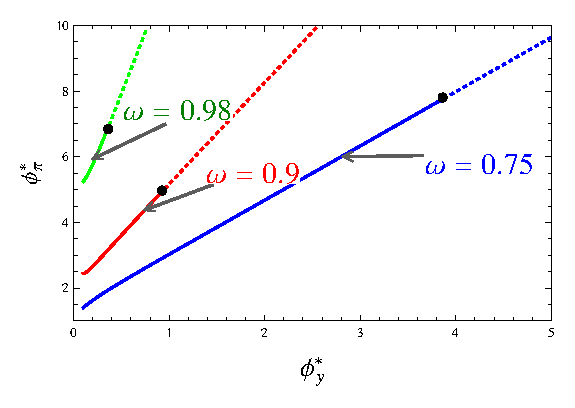
\includegraphics[width=3.2in]{optmanifomega.eps}}}
%   \end{center}
%   \caption{\label{optomega}  Optimal policies at the BLE with respect to $\omega$ (a) and corresponding optimal manifolds for three different $\omega$ (connection points of solid and dotted curves corresponding to finite optimal policies) (b) with the contemporaneous interest rate rule. Parameters are: $\lambda=0.99, \varphi=1, \gamma=0.04,\frac{\sigma_2}{\sigma_1}=0.5$ and $\rho=0.5$.}
%    \end{figure}



\begin{figure}
    \begin{center}
        \mbox{\subfigure[Optimal manifold]
        {\includegraphics[width=3.2in]{optpolicy.eps}}\quad
        \subfigure[Loss function along optimal manifold]
         {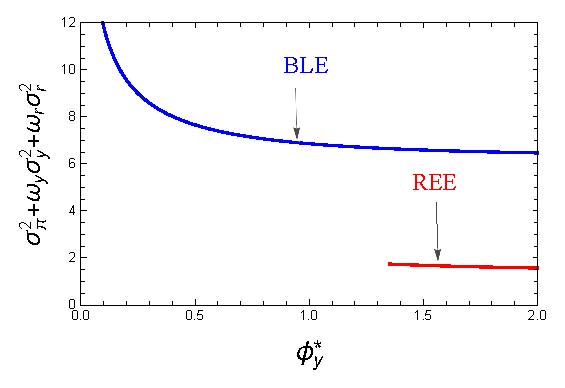
\includegraphics[width=3.2in]{optimalvar.eps}}}
   \end{center}
   \caption{\label{optbench} Optimal manifolds at the BLE and REE given each $\phi_y^*$ (a) and the corresponding loss function along the optimal paths (b) with the contemporaneous interest rate rule. Parameters are: $\lambda=0.99, \varphi=1, \gamma=0.04,\sigma_1=1,\sigma_2=0.5$ and $\omega_y=1,\omega_r=0.05$.}
    \end{figure}


\newpage




\end{document}
